\appendix{}

\section{Setup of GP model training}\label{app:A}

This section includes detailed discussions about the selections of mean function, likelihood and loss function, optimiser, and early stopping. 

\subsection{Mean Function}

We first investigate the mean function. As discussed above, the data distribution is generally smooth but complex in some regions of parameter space (e.g., the sub-giant hook).  Although a GP model can cope with different mean functions,  because of the flexibility of kernels, we find that using a constant or a linear mean function leads to a long time for training. For this reason, we apply a Neural Network mean function which is flexible enough to manage both simple and complex features. We adopt an architecture including 6 hidden layers and 128 nodes per layer. All layers apply the linear transformation to the incoming data. We apply the element-wise function (Elu) because it give relatively smooth mean functions. ({\bf Can Guy or Alex add some references for NN and Elu here? The referee may ask why the 6x128 architecture is sufficient, so should we mention Alex's paper?})

\subsection{Likelihood and Loss Function}

Our training dataset is a theoretical model grid,  hence there is no observed uncertainty for each data point, but a tiny random uncertainty exists due to the approximations in the \textsc{MESA} numerical method. We model this using $\sigma_{w}$.  This noise model is then assumed to be a Gaussian function with a very small variance.  
%   
A likelihood specifies the mapping from input values $f(X)$ to observed labels $y$.
We adopt the the standard likelihood for regression which assumes a standard homoskedastic noise model whose conditional distribution is
\begin{equation}\label{eq:likelihood}
p(y|f(x)) = f + \epsilon, \epsilon \sim \mathcal{N}(0, \sigma^{2}),
\end{equation}
where $\sigma$ is a noise parameter. 
%
We used a small and fixed noise parameter and run a few tests.  However, the strict noise parameter makes GP models hard to converge. When this noise parameter is set as free, it reduces to a small value anyway in the training progress because it is data-driven.  For this reason, we did not put strict constraint for or prioritise this noise parameter.  In practice, we only set up a loose upper limit ($\sigma$  < 0.1) to speed up the training. One thing should be noted that a GP model with a large noise parameter is not a proper description for the stellar grid. Because of this, we only adopt GP models with $\sigma$ $\lesssim 10^{-4}$. We train GP models model using the negative logarithm of the likelihood function as the loss function.  

\subsection{Optimiser}

We compared two optimisers named SGD and Adam. Here SGD refers to Stochastic Gradient Descent, and Adam is a combination of the advantages of two other extensions of stochastic gradient descent, specifically, Adaptive Gradient Algorithm and Root Mean Square Propagation. 
%
The SGD optimiser in the \textsc{GPyTroch} package involves the formula given by \citet{sutskever2013importance}. The formula makes it possible to train using stochastic gradient descent with momentum thanks to a well-designed random initialisation and a particular type of slowly increasing schedule for the momentum parameter. The application of momentum in SGD could improve its efficiency and make it less likely to stuck in local minimums. On the other hand, the Adam optimiser includes the 'AMSGrad' variant developed by \citet{47409} to improve its weakness in the convergence to an optimal solution. With these new developments, the two optimisers give very similar results. We finally choose Adam because it works relatively efficiently and stable.  
%
We adaptive learning rate in the training process. Our training starts with a learning rate of 0.01 and decreases by a factor of 2 when the loss value does not reduce in previous 100 iterations.    

\subsection{Early Stopping}

We set up an Early Stopping for avoiding overfitting and also determining when to terminate a training progress. 
When an optimal solution is found, the validating errors stop decreasing and then increase when overfitting occurs. 
We hence track down the validating error every iteration and terminate training process when the validating error does not decrease in previous 300 iterations. 	

\section{State-of-the-art implement for large dataset}\label{app:B}

In section \ref{sec:3d}, we investigate the strategy for large dataset. We test two State-of-the-art approaches that designed for training big data whose data size is more than the limit of a GP model. Here we mention some details about the two methods and the results. 

We first consider the Stochastic Variational GP (SVGP) approach based on the \textsc{GPyTorch ApproximateGP} module. 
We train our data based on the SVGP example on \url{https://docs.gpytorch.ai/en/v1.1.1/examples/04_Variational_and_Approximate_GPs/SVGP_Regression_CUDA.html}. 
SVGP is an approximate scheme rely on the use of a series of inducing points which can be selected in the parameter space. It trains using mini batches and hence is able to deal with large data size. The other key point of SVGP is the number of inducing points. Because the kernel is only built on these points, the number determines the complexity of kernel. When the underline function is simple, for instance, a power law, a small number of inducing points  is enough. For our application, a large number of inducing points are required. Underline principles and detailed descriptions of this approach can be found in \citet{hensman2015scalable}. In our tests on 3D problem, we find a practical issue with the SVGP approach. When we load in a large training sample which takes a lot GPU memory, the rest memory can capacitate only 10,000 inducing points. This is to say, we use more training data but sacrifice the kernel complexity.  The result shows that using SVGP model does not improve the GP predictions compared with normal GP model. For instance, the 68th, 95th, and 99.7th testing errors for $T_{\rm eff}$ are 2.2, 6.8, and 15.1K (EI = 24.1 K) for the SVGP and 2.0, 5.8, and 15.7 K (EI = 23.5K) for the normal GP model. This is because the evolutionary feature are complex across multiple demissions. Reducing the kernel complexity is not ideal. We conclude that the SVGP is suitable for training large data which have relatively simple variations but not a good choice for training the model grid.  

We also investigate another approach designed for large dataset named Structured Kernel Interpolation (SKI GP). SKI GP was introduced by \citet{wilson2015kernel}. It produces kernel approximations for fast computations through kernel interpolation and is a great way to scale a GP up to very large datasets (100,000+ data points).
We follow the example on \url{https://docs.gpytorch.ai/en/stable/examples/02_Scalable_Exact_GPs/KISSGP_Regression.html} to develop our script. 
We run a few tests to train a 3D SKI GP model with 100, 000 training data. Compare with the Normal GP and SVGP, its testing errors for $T_{\rm eff}$ are slightly improved to 2.0, 6.1, and 14.8K (EI = 22.9K). However, the further test on the 5-demission data is not ideal: a SKI GP model using 100, 000 training data performs much worse than a normal model with only 20,000 training data. The poor behaviour consists with what has been discussed by \citet{wilson2015kernel}: the SKI GP poorly scale to data with high dimensions, since the cost of creating the grid grows exponentially in the amount of data. We attempt to make some additional approximations with the \textsc{GpyTorch AdditiveStructureKernel} module. It makes the base kernel to act as one-dimension kernels on each data dimension and the final kernel matrix will be a sum of these 1D kernel matrices. However, the testing errors are not significantly improved. 

%\begin{figure}
%	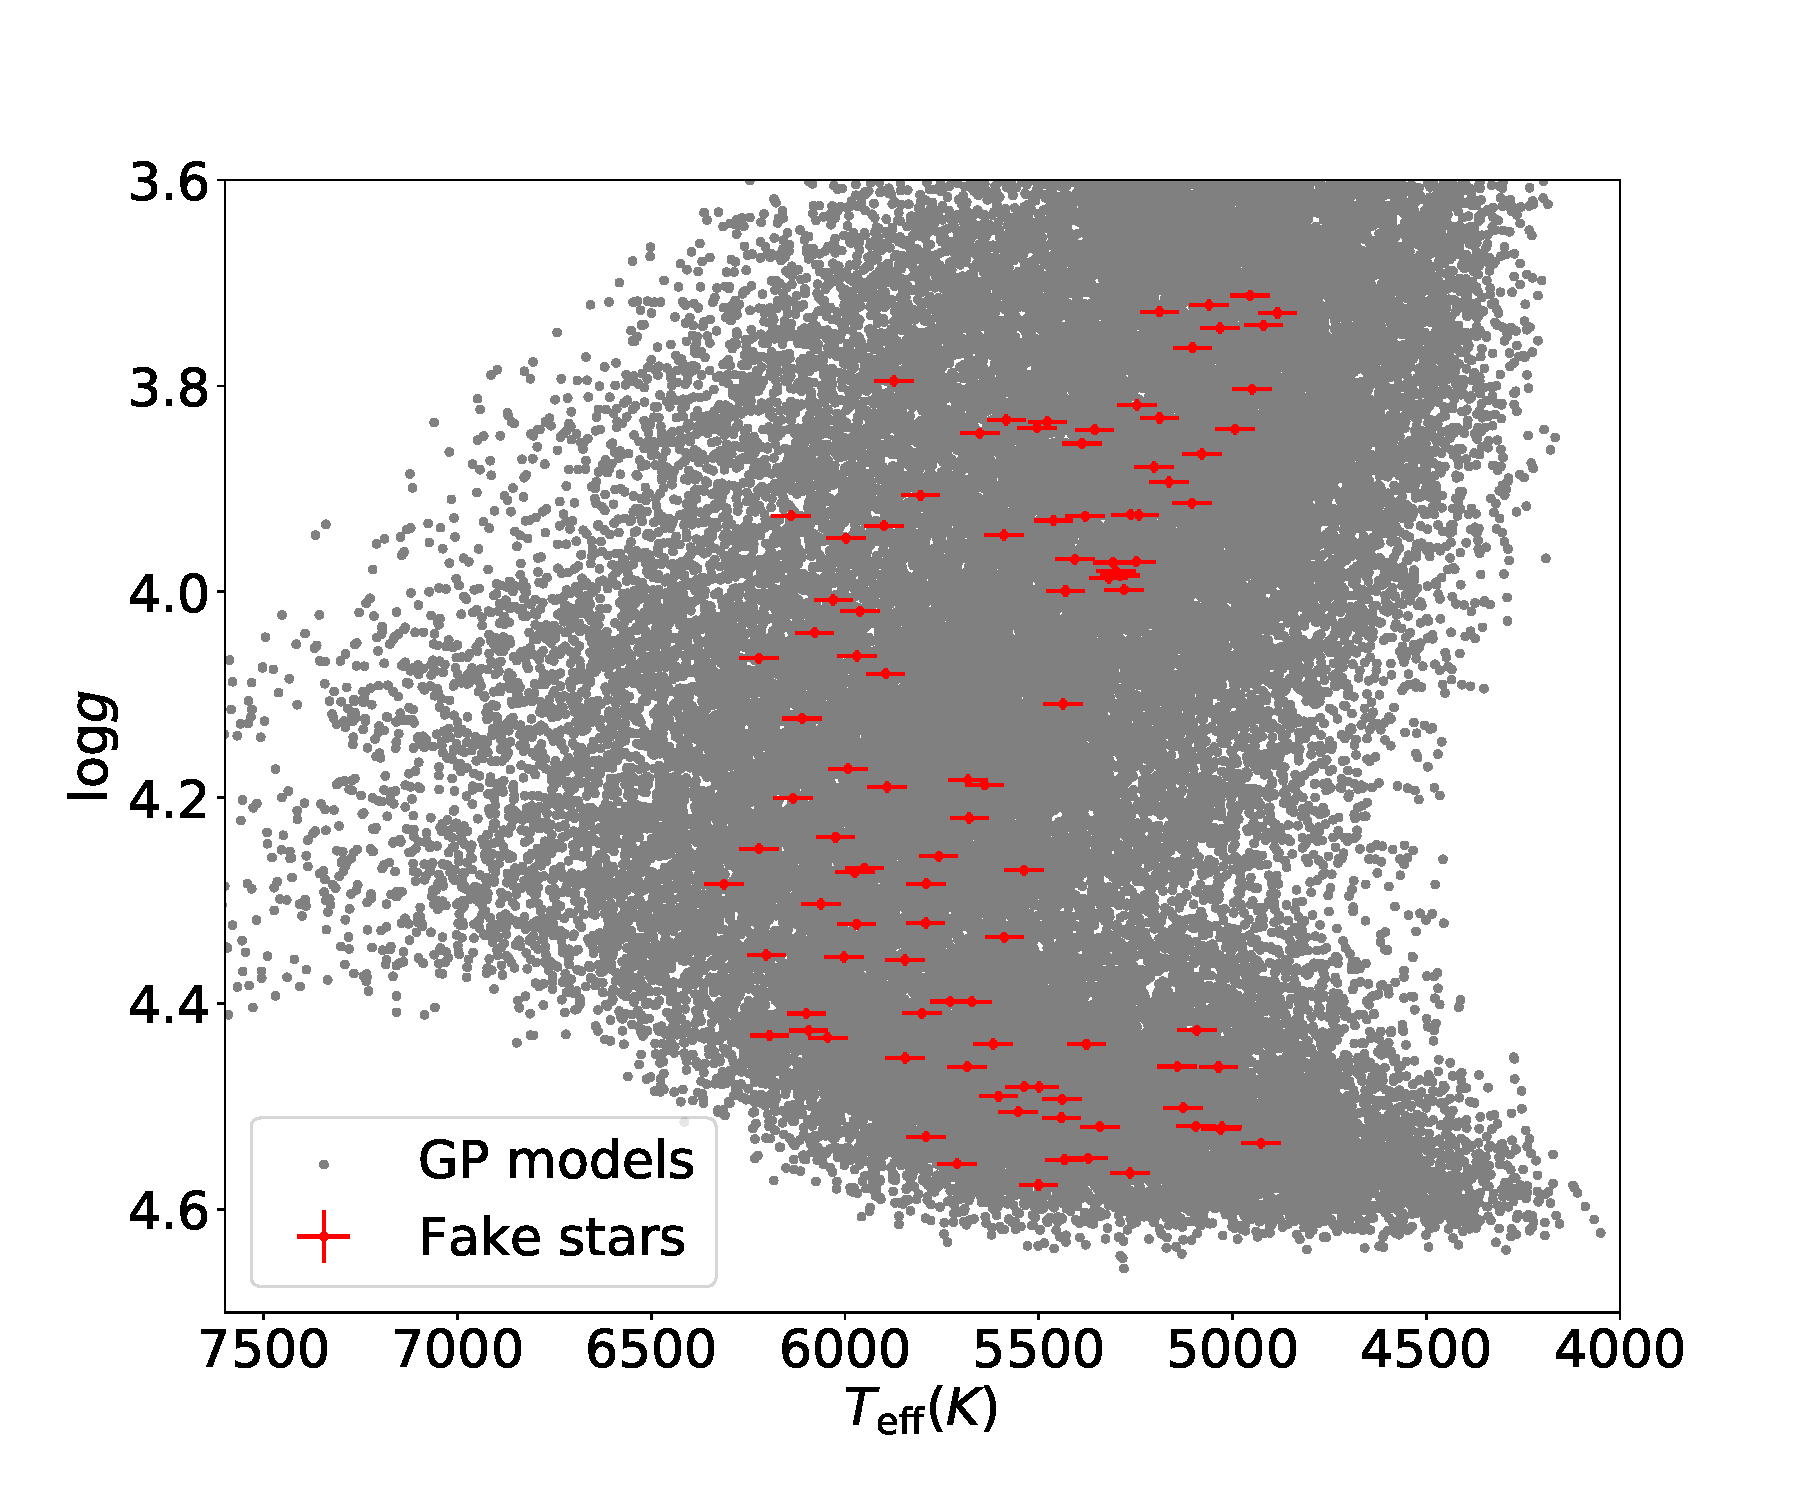
\includegraphics[width=1.0\columnwidth]{fake-stars-on-hrd.pdf}
%    \caption{Fake stars on the Keil diagram. } 
 % \label{fig:fit_comparison}
%\end{figure}




